% !TEX root = main.tex

\section{调度}
\subsection{单处理器调度}
三级调度层次
\begin{itemize}
    \item 长程调度(Long-term scheduling)/任务调度
    \begin{itemize}
    \item 决定哪些新建进程可进入系统\textbf{准备执行}(ready)
    \item 控制多道程序系统的并发程度
    \item 进程越多则各进程对CPU的使用百分比越小
    \end{itemize}
    \item 中程调度(Medium-term scheduling)
    \begin{itemize}
    \item 决定交换哪些主存-辅存(内存-外存)进程
    \item 基于多道程序设计的管理需要
    \end{itemize}
    \item 短程调度(Short-term scheduling)/CPU调度
    \begin{itemize}
    \item 决定下一个使用CPU的进程(dispatcher,分派程序)
    \end{itemize}
\end{itemize}

\begin{figure}[H]
    \centering
    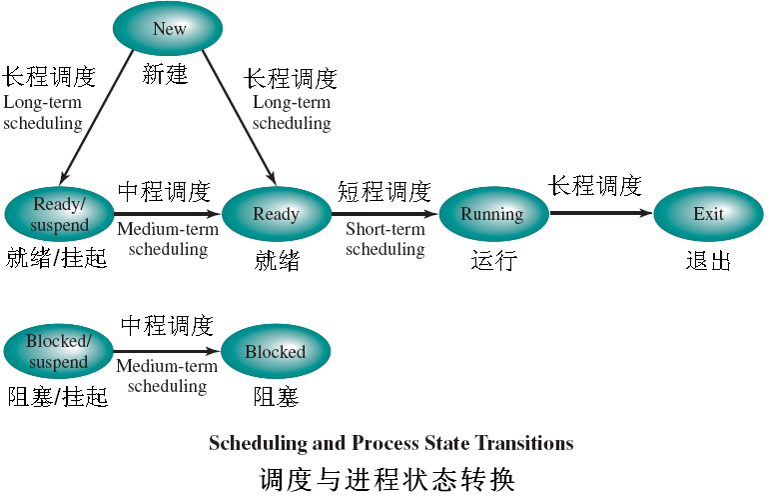
\includegraphics[width=0.6\linewidth]{fig/process_scheduling.png}
\end{figure}

进程调度方式
\begin{itemize}
    \item 剥夺式:立即分配
    \item 非剥夺式:当前进程执行完再分配给新进程
\end{itemize}

进程调度算法
\begin{itemize}
\item 先来先服务(First Come First Served,FCFS):公平
\item 最短进程优先(Shortest Process Next,SPN):效率,EWMA
\[S_{n+1}=aT_n+(1-a)S_n\]
\item 最短剩余优先(Shortest Remaining Time,SRT)
\item 最高响应比优先(Highest Response Ratio Next,HRRN)
\[R_P=\frac{T_{wait}+T_{serve}}{T_{serve}}\]
\item 时间片(time slicing)轮转(Round Robin,RR)
\item 最高优先级优先(Highest Priority First,HPF)
\item 多级队列反馈(Multilevel Feedback,MF/FB)
\end{itemize}

周转时间:作业提交到作业完成所经历的时间

\subsection{多处理器调度}
多处理器线程调度方案
\begin{itemize}
    \item 负载共享(load sharing)
    \item 组调度(gang scheduling)
    \item 专用处理器分配
    \item 动态调度
\end{itemize}

% 填空10*2
% 简答题6*5
% 应用题5